\subsection{Ride Manager}
\begin{figure}[H]
	\centering
	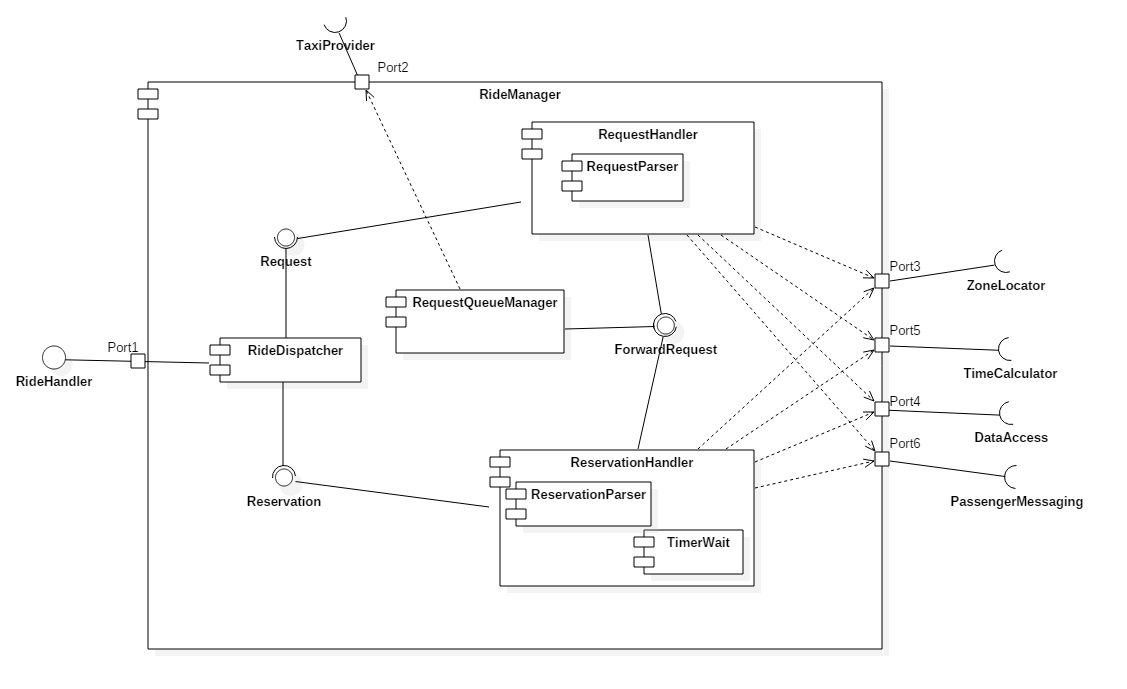
\includegraphics[trim=50 0 0 0,scale=0.45]{../"Analysis Documents"/components/ridemanager}
	\label{fig:rideHandler}
	\caption{Ride Handler}
\end{figure}
\subsubsection{Provided interfaces}
\begin{table}[H]
\begin{longtable}{| p{0.3\textwidth} | p{0.3\textwidth} | p{0.4\textwidth} |}
\hline
 \textbf{Provided Interface} & \textbf{Dedicated user} & \textbf{Description} \\ \hline
RideHandler & The Passenger's application and the relative web application & Login, logout, registration and deletion of the account \\ \hline
\end{longtable}
\caption{Ride Handler: provided interfaces}
\label{tab:rideHandler:providedInterfaces}
\end{table}
\subsubsection{Required interfaces}
\begin{table}[H]
\begin{longtable}{| l | p{.80\textwidth} |}
\hline
 \textbf{Required Interface} & \textbf{Description and usage} \\ \hline
DataAccess & Access to the data layer in order to 
			\begin{itemize}
				\item Store data of the request
				\item Store data of the reservation
				\item Retrieve reservations in order to forward them to the TaxiManager
			\end{itemize} \\ \hline
Zone Locator & Check the correctness of the location data provided by the user \\ \hline
TaxiProvider & Retrieve a taxi who accepted the request/reservation or an error message saying the nature of the problem. \\ \hline
\end{longtable}
\caption{Ride Handler: required interfaces}
\label{tab:rideHandler:requiredInterfaces}
\end{table}
